\section{Basic Creation Tools}
\label{prototype:BasicCreationTools}
I’ve made a small but useful update: adding notes and tags is now easily accessible via a UI button.

While this enhancement might seem minor, it has highlighted some backend logic issues that need to be addressed. Ideally, every time a change is made, the entire representation should refresh to display all updated information accurately. However, this approach creates a jarring user experience, with elements “popping in,” disappearing, or shifting unexpectedly.

Currently, this implementation creates a new node on the front end (placing it at a default position on the map) and then communicates with the backend to save the data. While functional under normal circumstances, this approach has some significant drawbacks. For instance, if the database is modified while a user is working, there’s a risk of data loss or corruption. Additionally, this method complicates real-time collaboration between multiple users, as they would need to refresh their pages frequently to stay in sync - clearly a poor solution.

In future iterations I will need to address this, potentially by re-engineering all communication between client and server.

\begin{figure}[H]
\centering
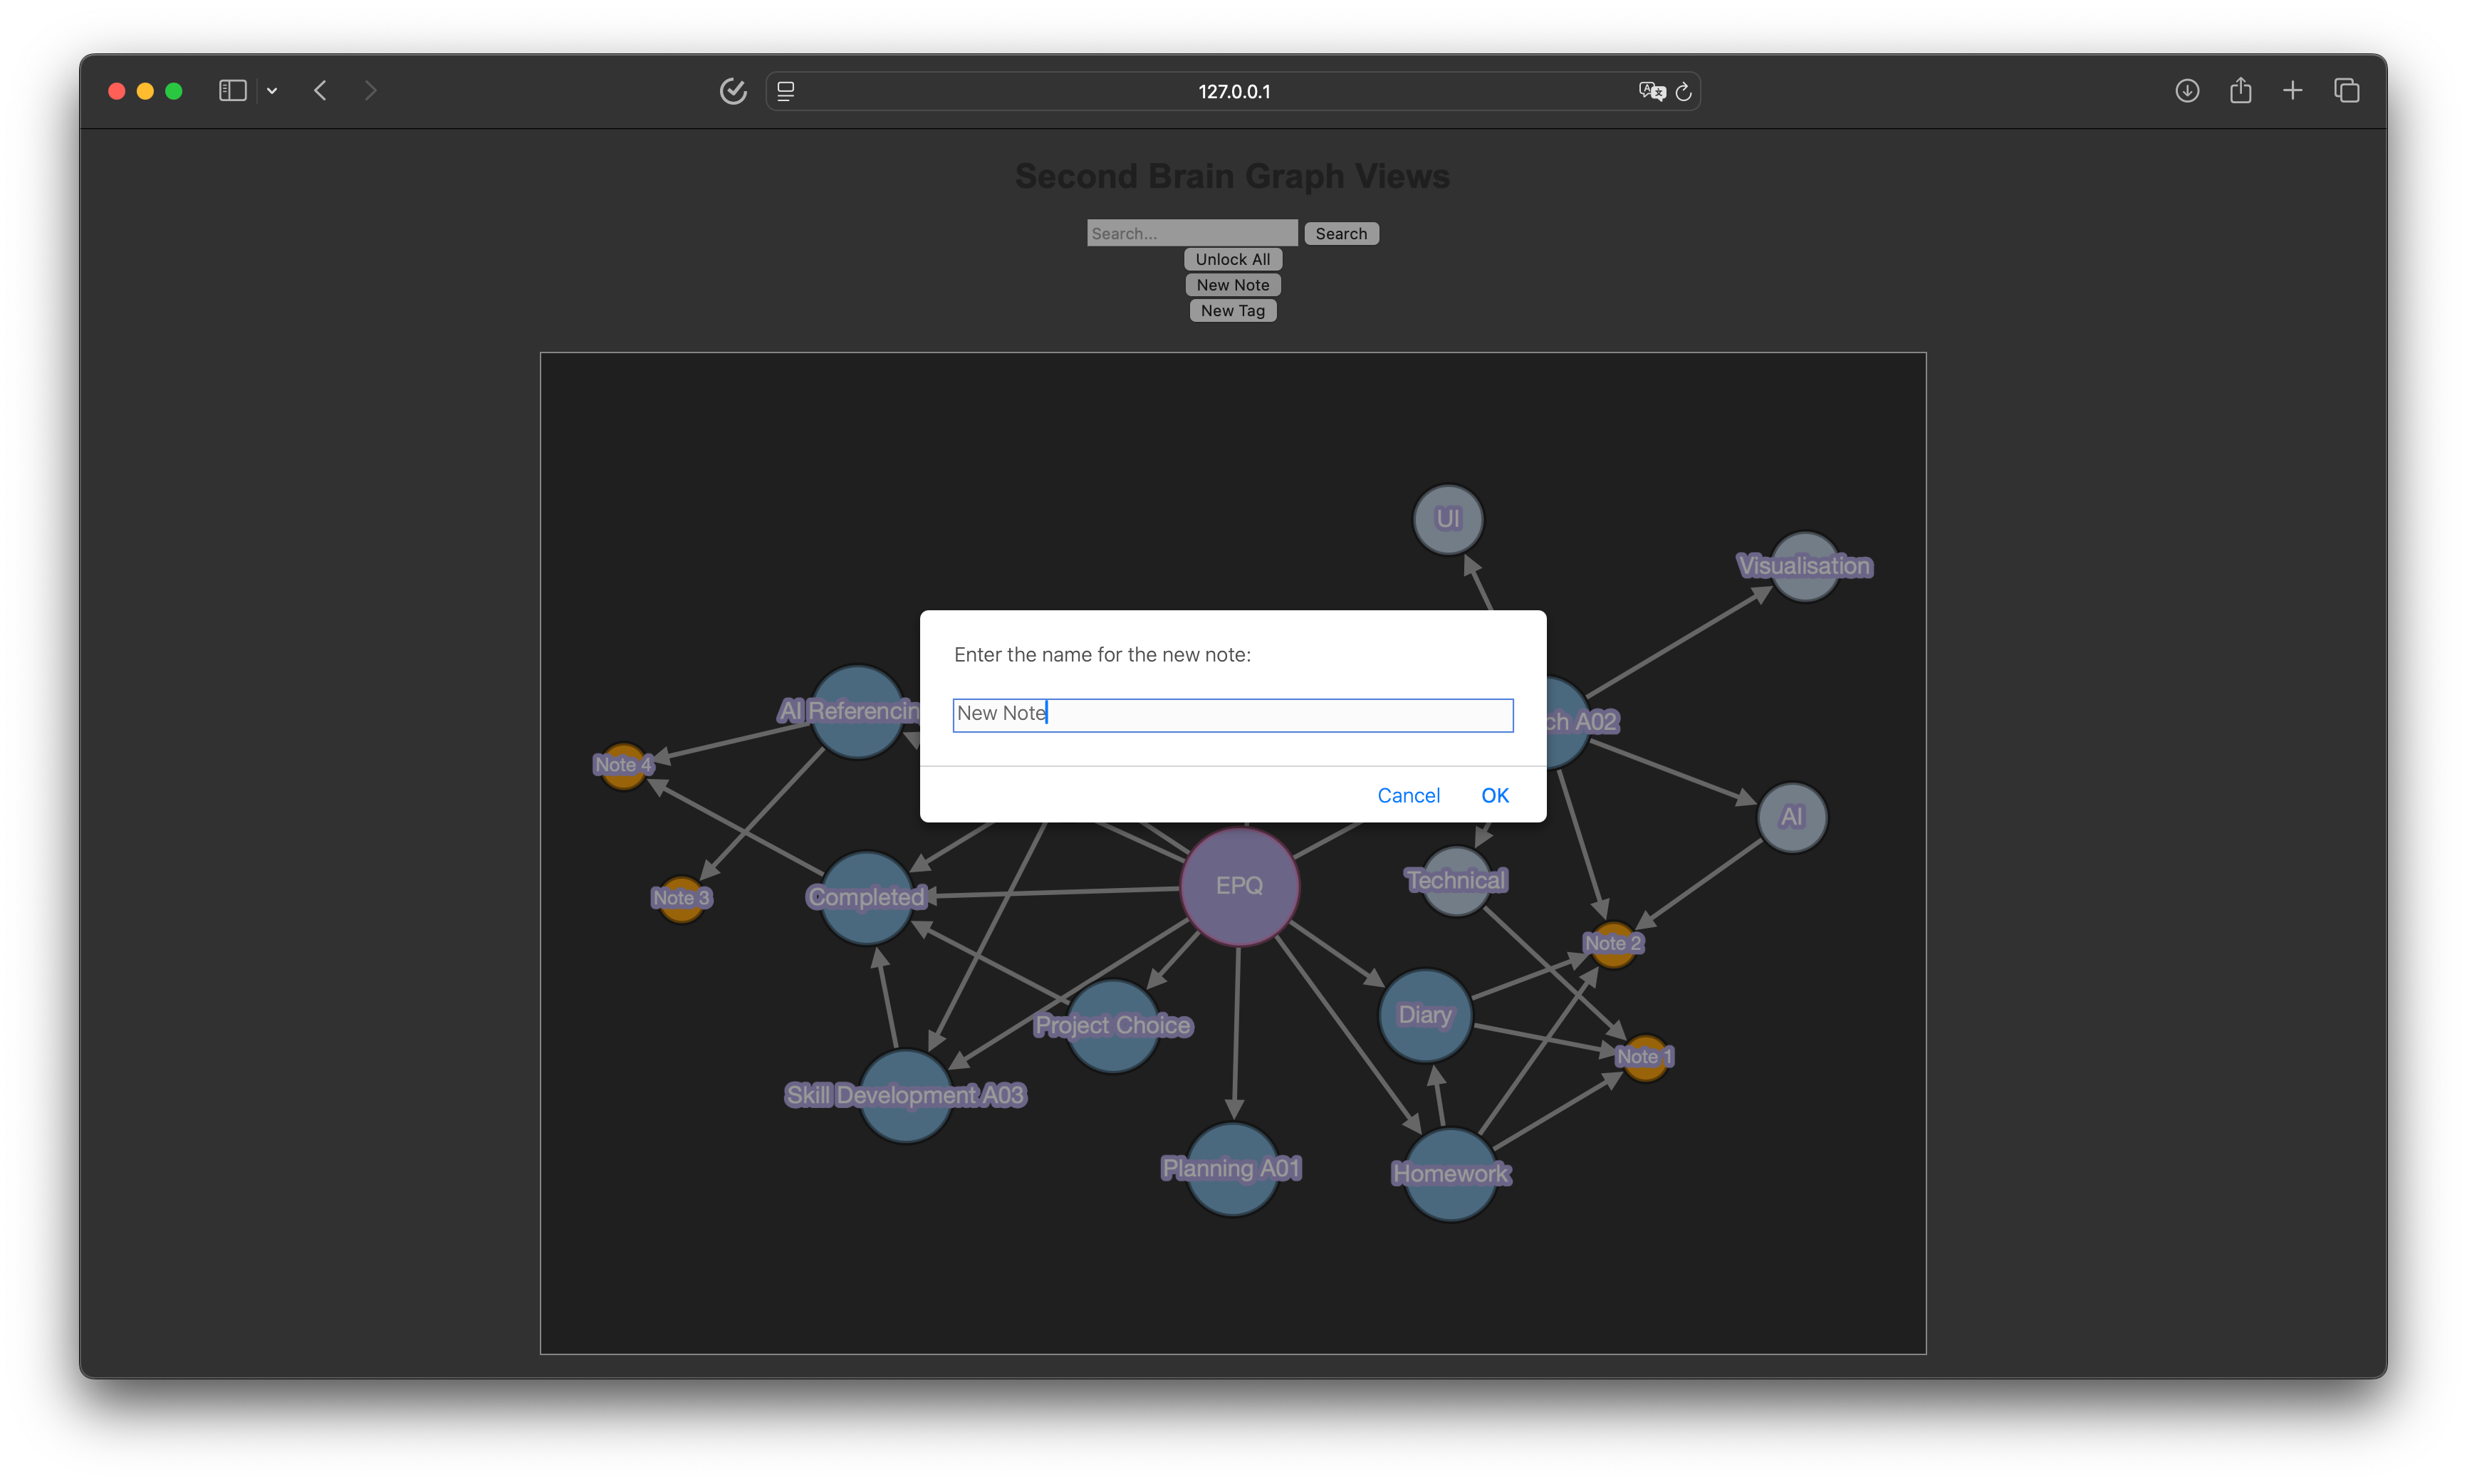
\includegraphics[width=0.8\textwidth]{Prototype/10_BasicCreationTools/media/prototype.png}
\caption{My basic creation tool prototype}
\end{figure}